\documentclass{article}
\PassOptionsToPackage{colorlinks=true, allcolors=blue}{hyperref}

\usepackage[preprint]{neurips_2026}


\usepackage{fontspec}
\usepackage{hyperref}       % hyperlinks
\usepackage{url}            % simple URL typesetting
\usepackage{booktabs}       % professional-quality tables
\usepackage{amsfonts}       % blackboard math symbols
\usepackage{amsmath}        % math environments
\usepackage{amssymb}        % math symbols
\usepackage{nicefrac}       % compact symbols for 1/2, etc.
\usepackage{microtype}      % microtypography
\usepackage[svgnames]{xcolor} % colors
\usepackage{graphicx}       % graphics
\usepackage{listings}       % code listings
\usepackage{multirow}
\usepackage{float}
\usepackage[frozencache]{minted}
\usepackage{csquotes}

% --- TikZ for diagrams ---
\usepackage{tikz}
\usetikzlibrary{shapes.geometric, arrows.meta, positioning, fit, backgrounds, calc}
\usepackage{pgfplots}
\pgfplotsset{compat=1.18}

% For figures.
\usepackage{wrapfig}


\usepackage[disable]{todonotes}
\usepackage{comment}
\setuptodonotes{color=blue!30, fancyline}

\newmintinline[lean]{lean4}{breaklines,breakbefore={. },breakafter={_}}
\newminted[leancode]{lean4}{autogobble}

% JuliaMono has all the symbols needed for Lean code
\setmonofont[Scale=MatchLowercase]{JuliaMono}[
  Extension=.ttf,
  UprightFont=*-Regular,
  BoldFont=*-Bold,
  ItalicFont=*-RegularItalic,
  BoldItalicFont=*-BoldItalic,
  RawFeature={-calt},
]


% color already provided by xcolor above
\definecolor{keywordcolor}{rgb}{0.7, 0.1, 0.1}   % red
\definecolor{tacticcolor}{rgb}{0.0, 0.1, 0.6}    % blue
\definecolor{commentcolor}{rgb}{0.4, 0.4, 0.4}   % grey
\definecolor{symbolcolor}{rgb}{0.0, 0.1, 0.6}    % blue
\definecolor{sortcolor}{rgb}{0.1, 0.5, 0.1}      % green
\definecolor{attributecolor}{rgb}{0.7, 0.1, 0.1} % red

\def\lstlanguagefiles{lstlean.tex}
% set default language
\lstset{language=lean, escapeinside={(*}{*)}}

% below: to typeset diffs
  \definecolor{diffstart}{named}{Grey}
  \definecolor{diffincl}{named}{Green}
  \definecolor{diffrem}{named}{OrangeRed}
  \lstdefinelanguage{diff}{
    basicstyle=\ttfamily\small,
    morecomment=[f][\color{diffstart}]{@@},
    morecomment=[f][\color{diffincl}]{+ },
    morecomment=[f][\color{diffrem}]{- },
  }

\title{Formal Conjectures: An Open and Evolving Benchmark for Verified Discovery in Mathematics}

\author{%
  \textbf{Moritz Firsching}$^1$\thanks{Equal contribution. Correspondence to: \texttt{firsching@google.com}} \quad
  \textbf{Paul Lezeau}$^2$\footnotemark[1] \quad
  \textbf{Salvatore Mercuri}$^2$\footnotemark[1] \quad
  \textbf{Mikl\'{o}s Z.~Horv\'{a}th}$^1$\footnotemark[1] \\
  \textbf{Ya\"{e}l Dillies}$^3$ \quad
  \textbf{Calle S\"{o}nne}$^1$ \quad
  \textbf{Eric Wieser}$^1$ \quad
  \textbf{Fred Zhang}$^1$ \\
  \textbf{Thomas Hubert}$^1$ \quad
  \textbf{Blaise Ag\"{u}era y Arcas}$^4$ \quad
  \textbf{Pushmeet Kohli}$^1$ \\
  \vspace{0.1cm} \\
  $^1$Google DeepMind \quad $^2$Imperial College London \quad
  $^3$Stockholms universitet \quad $^4$Google
}






\begin{document}


\maketitle


% Auto-generated by scripts/generate_tables.py — do not edit by hand.
\newcommand{\fcCountTotal}{2615}
\newcommand{\fcCountResearchOpen}{1029}
\newcommand{\fcCountResearchSolved}{836}
\newcommand{\fcCountTest}{467}
\newcommand{\fcCountAPI}{155}
\newcommand{\fcCountTextbook}{128}
\newcommand{\fcCountSolvedGroup}{964}
\newcommand{\fcCountInfraGroup}{622}
\newcommand{\fcCountAllOther}{750}
\newcommand{\fcCountInfraPct}{23.8}
\newcommand{\fcSrcErdos}{1318}
\newcommand{\fcSrcWikipedia}{476}
\newcommand{\fcSrcGreens}{175}
\newcommand{\fcSrcPapers}{131}
\newcommand{\fcSrcOQP}{125}
\newcommand{\fcSrcWOWII}{110}
\newcommand{\fcSrcOEIS}{105}
\newcommand{\fcSrcArxiv}{56}
\newcommand{\fcSrcMO}{53}
\newcommand{\fcSrcOther}{66}

\begin{abstract}
As automated reasoning systems advance rapidly, there is a growing need for research-level formal mathematical problems to accurately evaluate their capabilities.
To address this, we present Formal Conjectures,\footnote{\url{https://github.com/google-deepmind/formal-conjectures}} an evolving benchmark of currently \fcCountTotal{} mathematical problem statements formalized in Lean~4.
Sourced from areas of active mathematical research, the dataset features \fcCountResearchOpen{} open research conjectures providing a zero-contamination benchmark for mathematical proof discovery, and \fcCountResearchSolved{} solved problems for proof auto-formalization.
Notably, the repository provides a structured interface connecting mathematicians who formalize and clarify problems with the AI systems and humans attempting to solve them.
Demonstrating its immediate utility, the benchmark has already been leveraged to make new mathematical discoveries, including the resolution of open research conjectures.
We describe our approach to ensuring the correctness of these formalizations in a collaborative open-source project where contributions stem from an active community.
In this framework, AI-generated proofs and disproofs serve as a valuable auditing mechanism to iteratively improve the fidelity of the benchmark.
Finally, we provide a standardized evaluation setup and report baseline results on frozen evaluation subsets, demonstrating a climbable signal that measures the current frontier of automated reasoning on research-level mathematics.
\end{abstract}


\section{Introduction}\label{sec:introduction}


As automated reasoning systems, including large language models (LLMs), continue improving their capabilities, the benchmarks used to measure their progress face significant challenges.
In the domain of (formal) mathematics, many existing evaluation frameworks suffer from: \textbf{(i) Data leakage:} As solutions to benchmark problems appear online, it is difficult to distinguish genuine reasoning from memorization. This is a challenge for benchmarks like \cite{minif2f21, putnambench24, jiang2025fate, yu2025formalmath}; \textbf{(ii) Secretive evaluation:} To combat leakage, some benchmarks require that the evaluation set be kept private, which hinders open and reproducible research \citep{ARC24, frontiermath24, humanitysexam25}; \textbf{(iii) Oversimplified success criteria:} Many benchmarks rely on verifying a simple, machine-checkable final answer (such as a number), which fails to capture the complex, multi-step reasoning inherent in a full mathematical proof \citep{hendrycks2measuring, frontiermath24}; and \textbf{(iv) Saturation:} As models improve, some benchmarks become saturated. For instance, MiniF2F \citep{minif2f21} is now routinely solved with over 99\%; see \cite{AlphaProof25, chen2025seed, lin2025goedelproverv2}.


To address these limitations, we introduce \textbf{Formal Conjectures}, an open-source and growing collection of mathematical problems formalized in Lean~4 \citep{moura2021lean} using Mathlib \citep{mathlib2020}.
The benchmark focuses on \emph{open conjectures} as the primary challenge, providing a zero-contamination testbed where solutions cannot be found in existing training data.
The secondary challenge consists of (informally) solved problems for auto-formalization, which do not share the same zero-contamination guarantees.
We formalize all problems in a formal language to allow for objective, rigorous, and automated evaluation: a proposed solution is definitively correct if and only if its corresponding proof is accepted by the kernel without relying on forbidden axioms like \lstinline{sorry}.
Our choice of Lean~4 is pragmatic: Mathlib, the largest formal mathematics library available, is essential for stating a wide variety of advanced conjectures.
While we focus on Lean~4, the core principles of our benchmark are language-agnostic and extendable to other formal systems. %, as discussed in Section \ref{sec:discussion}.


This paper details the construction and methodology of the \textbf{Formal Conjectures} benchmark.
The benchmark is publicly available under the Apache 2.0 license and has already been utilized for real-world mathematical discovery \citep{alexeev25, DMProverAgent26}. In summary, our main contributions are:
\begin{itemize}
    \item \textbf{The Formal Conjectures Benchmark:} A large-scale, evolving dataset of \fcCountTotal{} mathematical statements in Lean~4, including \fcCountResearchOpen{} open conjectures for zero-contamination proof discovery and \fcCountResearchSolved{} solved problems for auto-formalization.
    \item \textbf{A Unified API for Mathematical Reasoning:} A repository interface connecting mathematicians with an ecosystem of automated solvers to facilitate simultaneous statement auditing and rapid dissemination of problems to AI systems.
    \item \textbf{Methodology for Statement Formalization:} We introduce a collaborative pipeline and a three-level taxonomy of misformalizations (Translation, Underspecified, and Source) to ensure formalization fidelity. This includes the \texttt{answer(sorry)} mechanism, which decouples the mathematical value discovery from proof verification. We provide insights from 291 fixed cases of research-level formalization.
    \item \textbf{A Standardized Evaluation Framework:} We provide a rigorous evaluation setup using the Lean~4 kernel to verify multi-step reasoning without relying on oversimplified numerical answers. We establish frozen subsets, \texttt{FC100SolvedSet1} and \texttt{FC100OpenSet1}, to enable stable, reproducible model comparisons.
\end{itemize}



\section{Related Work}\label{sec:related_work}

Our work intersects mathematical reasoning benchmarks and formal theorem proving.

\paragraph{General mathematical reasoning benchmarks.}
Several benchmarks evaluate AI systems on advanced problem-solving without requiring formal proofs.
FrontierMath \citep{frontiermath24} uses expert-crafted problems verified by numerical answers, which, while machine-checkable, do not fully capture the multi-step reasoning process.
In January 2026, Epoch AI launched \emph{FrontierMath: Open Problems}, a website-only pilot of a small collection of unsolved research-level informal problems with evaluation offered as a service.
Humanity's Last Exam \citep{humanitysexam25} crowdsources expert questions but relies on answer-checking rather than proof verification.
MathArena \citep{matharena25} evaluates LLMs on fresh competition problems to reduce contamination risk and assesses informal proof-writing.
The ARC Prize \citep{ARC24, ARC25} targets abstract reasoning, sharing our focus on measuring genuine reasoning over pattern matching.
Formal benchmarks, by contrast, allow automatic verification of full reasoning or proof.

\paragraph{Formal mathematics benchmarks and automated theorem proving.}
Interest in automated theorem proving has accelerated AI reasoning, leading to the rapid saturation of existing formal benchmarks.
MiniF2F \citep{minif2f21} pioneered high-school-level evaluation but became increasingly saturated as models improved.
This shift was defined by AlphaProof \citep{AlphaProof25} and AlphaGeometry 2 \citep{chervonyi2025gold} reaching silver-medal performance at the 2024 IMO, where AlphaProof solved Lean problems and introduced the Formal-IMO \citep{AlphaProof25} dataset.
Systems like Aristotle \citep{achim2025aristotle} and Seed-Prover \citep{chen2025seed} achieved gold-medal equivalents at the 2025 IMO.
This capability leap cascaded to undergraduate math, where benchmarks like PutnamBench \citep{putnambench24} and Putnam 2025 are being saturated by models such as Seed-Prover 1.5 \citep{chen2025seed15} and Numina \citep{liu2026numina}, and other industry systems.
While SorryDB \citep{sorrydb26} evaluates AI on practical theorem completion and FATE \citep{jiang2025fate} targets varying difficulties of frontier algebra, the saturation of earlier benchmarks highlights an acute need for research-level evaluation: benchmarking reasoning on unsolved research-level mathematics.


\paragraph{Adoption of Formal Conjectures.}
Since its open-source release in May 2025, the repository has been adopted by both mathematicians and tool builders.
Boris Alexeev used a repository formalization to prove Erd\H{o}s Problem 124 \citep{erdos124} with Aristotle \citep{achim2025aristotle}.
Although the statement was initially misformalized and included an unintended extra hypothesis, Aristotle’s proof succeeded without relying on it.
Numerous subsequent successes such as \citep{alexeev25} highlight the repository’s value for discovery and demonstrate how AI-generated proofs serve as a vital auditing mechanism to improve formalization fidelity.
A DeepMind prover agent \citep{DMProverAgent26} conducted a systematic evaluation of the full repository, solving several open problems.
To facilitate standardized, reproducible evaluation, this paper introduces named, versioned snapshots (Section~\ref{sec:versioning}), moving beyond individual tests to systematic benchmarking across diverse methods.


\section{Formal Conjectures}\label{sec:formal_conjectures}

\subsection{Problem Selection and Composition}

\begin{figure}[t!]
    \centering
    \resizebox{\textwidth}{!}{
        \begin{tikzpicture}[
    font=\sffamily,
    % Background box styles
    boxgreen/.style={fill=green!5, draw=green!50!black, very thick, rounded corners=2ex},
    boxblue/.style={fill=cyan!5, draw=cyan!60!black, very thick, rounded corners=2ex},
    % Content box styles - REMOVED minimum height and tightened padding
    itembox/.style={rectangle, draw=black!25, fill=white, rounded corners=1ex, text width=9.2cm, inner sep=8pt, align=left, font=\sffamily\normalsize},
    repoitem/.style={rectangle, draw=cyan!40, fill=white, rounded corners=1ex, text width=9.2cm, inner sep=8pt, font=\sffamily\normalsize},
    % Arrows
    arrow/.style={thick, color=black!60, -{Stealth[scale=1.2]}}
]

    % ==========================================
    % 1. TOP LEFT: Informal Source Problems
    % ==========================================
    \node (source_title) [font=\sffamily\Large\bfseries, text=green!60!black] {Informal Source Problems};

    \node (src_all) [itembox, below=0.3cm of source_title] {
        \begin{tabular}{@{}lr@{}}
        Erd\H{o}s Problems                    & \fcSrcErdos \\
        Wikipedia                             & \fcSrcWikipedia \\
        Green's Open Problems                  & \fcSrcGreens \\
        Papers                                 & \fcSrcPapers \\
        Open Quantum Problems                  & \fcSrcOQP \\
        Written on the Wall II                 & \fcSrcWOWII \\
        OEIS                                   & \fcSrcOEIS \\
        arXiv                                  & \fcSrcArxiv \\
        MathOverflow                           & \fcSrcMO \\
        Other sources                          & \fcSrcOther \\
        \end{tabular}\\[2pt]
        \color{black!60} \small A mix of established archives, research collections, and open problem lists.
    };

    % ==========================================
    % 2. TOP RIGHT: Formal Conjectures Benchmark
    % ==========================================
    \node (repo_title) [font=\sffamily\Large\bfseries, text=cyan!80!black, right=5.2cm of source_title] {Formal Conjectures Benchmark};

    \node (repo_open) [repoitem, below=0.3cm of repo_title] {
        \textbf{\large Research Open (\fcCountResearchOpen)} \\
        \color{black!60} \small $\hookrightarrow$ Primary Goal: \textbf{New Proof Discovery} \\
        Zero-contamination testbed for genuine reasoning.
    };

    \node (repo_solved) [repoitem, below=0.2cm of repo_open] {
        \textbf{\large Research Solved (\fcCountResearchSolved)} \\
        \color{black!60} \small $\hookrightarrow$ Secondary Goal: \textbf{Auto-formalization}.
    };

    \node (repo_api) [repoitem, below=0.2cm of repo_solved] {
        \textbf{\large All Other Statements (\fcCountAllOther)} \\
        $\bullet$ Test (\fcCountTest) \quad $\bullet$ API (\fcCountAPI) \quad $\bullet$ Textbook (\fcCountTextbook)\\
        \color{black!60} \small $\hookrightarrow$ Purpose: \textbf{Sanity \& Definition Testing}.
    };

    % ==========================================
    % 3. FLOW ARROW & CENTRAL PIPELINE TEXT
    % ==========================================
    \begin{scope}[on background layer]
        \node (bg_inputs) [boxgreen, dashed, fit=(source_title) (src_all), inner sep=12pt] {};
        \node (bg_repo) [boxblue, dashed, fit=(repo_title) (repo_open) (repo_api), inner sep=12pt] {};
    \end{scope}

    % 1. Position label exactly in the middle between the two boxes at the bottom
    \node (pipeline_label) at ($(bg_inputs.south east)!0.5!(bg_repo.south west) + (0,-0.6cm)$) 
        [font=\sffamily\Large\bfseries, text=orange!90!black] {Formalization Pipeline};

    % 2. Draw a straight arrow connecting the boxes, positioned slightly above the label
    \draw [arrow, line width=1.8pt, color=orange!80!black] 
        (bg_inputs.east |- pipeline_label) ++(0,0.7cm) -- ($(bg_repo.west |- pipeline_label) + (0,0.7cm)$);
\end{tikzpicture}
    }
    \vspace{-10pt}
    \caption{Left: informal source distribution. Right: formal category distribution, including open (\fcCountResearchOpen) and solved (\fcCountResearchSolved) problems.}
    \label{fig:benchmark_pipeline}
\end{figure}


\begin{wrapfigure}{r}{0.4\textwidth}
  \centering
  \vspace{-20pt}
  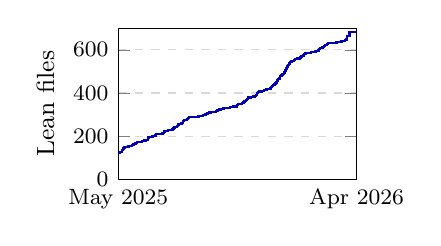
\begin{tikzpicture}
    \begin{axis}[
      width=0.38\textwidth,
      height=3.5cm,
      ymin=0, ymax=700,
      xmin=0, xmax=337.7,
      xtick={0,337.7},
      xticklabels={May 2025,Apr 2026},
      x tick label style={font=\footnotesize},
      ylabel={Lean files},
      ylabel style={font=\small},
      yticklabel style={font=\footnotesize},
      grid=major,
      grid style={dashed, gray!30},
      const plot,
    ]
    \addplot[blue!70!black, thick] coordinates {
        (0.00,122)
        (0.36,122)
        (0.42,122)
        (0.42,122)
        (0.43,122)
        (0.43,122)
        (0.45,122)
        (0.45,122)
        (0.46,122)
        (0.47,122)
        (0.48,122)
        (0.49,122)
        (0.50,122)
        (0.54,122)
        (0.62,122)
        (0.63,122)
        (0.64,122)
        (0.64,122)
        (0.68,122)
        (0.69,122)
        (0.71,122)
        (0.71,122)
        (0.72,122)
        (0.72,122)
        (0.72,122)
        (0.73,122)
        (1.37,122)
        (1.55,122)
        (1.66,122)
        (1.80,122)
        (1.94,122)
        (1.96,123)
        (1.97,124)
        (2.43,124)
        (2.44,124)
        (2.54,124)
        (2.75,125)
        (2.76,125)
        (3.92,126)
        (3.97,126)
        (4.54,126)
        (4.56,127)
        (4.60,127)
        (4.69,127)
        (4.74,128)
        (4.80,129)
        (5.43,129)
        (5.54,130)
        (5.55,131)
        (5.55,132)
        (5.57,133)
        (5.58,134)
        (5.84,135)
        (5.87,136)
        (5.95,136)
        (6.40,137)
        (6.46,138)
        (6.47,139)
        (6.51,139)
        (6.63,140)
        (6.68,140)
        (6.96,141)
        (7.38,142)
        (7.43,143)
        (7.51,143)
        (7.54,143)
        (7.65,144)
        (7.70,144)
        (8.41,144)
        (8.49,145)
        (8.62,146)
        (8.65,147)
        (8.71,148)
        (9.45,149)
        (9.46,149)
        (9.51,149)
        (9.72,149)
        (9.93,149)
        (10.72,149)
        (10.74,149)
        (11.89,149)
        (13.74,150)
        (13.79,151)
        (13.97,152)
        (14.52,153)
        (14.68,154)
        (15.40,154)
        (15.43,155)
        (15.58,155)
        (16.68,156)
        (19.50,157)
        (19.50,158)
        (20.43,158)
        (20.44,159)
        (20.54,160)
        (21.34,161)
        (21.55,162)
        (21.55,163)
        (22.54,164)
        (23.52,165)
        (23.58,166)
        (24.50,167)
        (26.45,168)
        (26.47,171)
        (27.60,172)
        (27.60,172)
        (28.73,172)
        (28.77,172)
        (29.54,172)
        (29.58,172)
        (29.60,172)
        (29.60,172)
        (29.69,172)
        (29.72,172)
        (29.73,172)
        (29.73,172)
        (29.79,173)
        (31.84,173)
        (31.84,174)
        (33.59,175)
        (33.59,176)
        (33.65,176)
        (34.87,177)
        (35.18,177)
        (35.39,177)
        (36.41,179)
        (36.97,179)
        (37.31,180)
        (37.43,180)
        (37.52,180)
        (39.58,181)
        (39.68,181)
        (41.44,182)
        (41.82,183)
        (42.52,183)
        (42.55,184)
        (42.63,184)
        (42.65,184)
        (42.71,194)
        (42.76,195)
        (42.87,195)
        (43.44,195)
        (43.45,195)
        (43.76,195)
        (44.40,195)
        (44.45,195)
        (44.45,195)
        (47.35,196)
        (47.56,197)
        (48.46,198)
        (48.64,198)
        (48.67,198)
        (49.49,199)
        (49.97,200)
        (50.37,200)
        (50.37,200)
        (50.47,200)
        (50.53,201)
        (51.64,202)
        (51.72,203)
        (52.66,204)
        (53.30,205)
        (53.43,206)
        (53.43,207)
        (53.44,208)
        (54.63,208)
        (55.29,209)
        (55.49,209)
        (55.49,210)
        (61.51,211)
        (62.70,212)
        (62.77,213)
        (63.43,215)
        (63.62,216)
        (64.38,217)
        (64.48,219)
        (64.51,219)
        (64.57,220)
        (64.65,220)
        (64.66,221)
        (64.74,221)
        (65.44,221)
        (65.46,222)
        (67.46,223)
        (67.56,224)
        (67.56,224)
        (68.47,225)
        (68.63,225)
        (68.72,225)
        (68.74,225)
        (68.79,225)
        (70.45,225)
        (70.50,225)
        (70.60,226)
        (70.63,227)
        (72.71,227)
        (74.58,228)
        (74.84,228)
        (74.84,228)
        (75.51,229)
        (75.57,229)
        (76.47,230)
        (76.67,231)
        (77.44,231)
        (77.54,232)
        (77.75,232)
        (77.75,232)
        (77.76,233)
        (77.76,233)
        (77.77,234)
        (77.79,234)
        (77.89,235)
        (78.45,235)
        (78.46,236)
        (78.47,236)
        (78.48,237)
        (78.60,238)
        (78.72,238)
        (78.87,238)
        (79.35,239)
        (79.66,240)
        (79.66,240)
        (79.73,241)
        (82.89,242)
        (83.38,244)
        (83.39,244)
        (83.40,245)
        (83.40,245)
        (83.51,245)
        (83.65,245)
        (83.69,248)
        (84.36,249)
        (84.56,250)
        (84.56,251)
        (84.66,252)
        (84.86,252)
        (84.86,253)
        (84.87,254)
        (85.38,254)
        (85.41,255)
        (85.68,255)
        (85.73,256)
        (86.29,256)
        (86.40,256)
        (86.40,256)
        (86.44,256)
        (87.44,257)
        (88.81,258)
        (90.35,259)
        (90.49,259)
        (90.52,259)
        (90.60,260)
        (91.40,260)
        (91.41,260)
        (91.41,261)
        (91.42,262)
        (91.43,263)
        (91.45,263)
        (91.46,264)
        (91.49,265)
        (91.52,266)
        (91.57,267)
        (91.62,267)
        (91.67,268)
        (91.72,269)
        (92.39,269)
        (92.42,269)
        (92.52,269)
        (92.59,269)
        (92.68,269)
        (92.75,269)
        (92.79,270)
        (92.90,270)
        (93.42,270)
        (93.44,271)
        (93.44,272)
        (93.66,272)
        (93.68,273)
        (96.45,273)
        (96.63,274)
        (96.65,274)
        (96.71,274)
        (96.76,274)
        (96.79,275)
        (96.94,276)
        (97.29,277)
        (97.31,278)
        (97.49,279)
        (98.44,279)
        (98.56,279)
        (98.65,280)
        (98.71,281)
        (98.78,282)
        (99.37,283)
        (99.44,284)
        (99.72,284)
        (100.47,284)
        (100.62,285)
        (100.64,286)
        (100.65,286)
        (100.74,286)
        (100.81,287)
        (100.82,288)
        (100.98,288)
        (101.15,288)
        (102.41,289)
        (103.39,289)
        (105.51,289)
        (105.53,289)
        (111.40,290)
        (113.35,291)
        (113.70,292)
        (118.79,293)
        (119.44,294)
        (119.62,294)
        (120.35,295)
        (120.36,296)
        (120.36,297)
        (120.52,297)
        (120.65,297)
        (120.69,298)
        (120.90,299)
        (123.35,300)
        (124.49,302)
        (124.77,303)
        (125.54,304)
        (125.61,305)
        (126.47,306)
        (127.33,307)
        (128.64,308)
        (128.66,309)
        (131.47,310)
        (131.47,311)
        (132.44,311)
        (134.55,311)
        (135.40,312)
        (136.51,313)
        (138.48,313)
        (138.49,313)
        (138.59,314)
        (138.63,315)
        (139.46,316)
        (139.49,317)
        (139.65,318)
        (140.55,319)
        (141.56,320)
        (142.48,321)
        (142.54,322)
        (142.57,322)
        (142.69,323)
        (145.51,324)
        (145.51,324)
        (145.51,324)
        (146.40,325)
        (146.45,326)
        (146.56,326)
        (146.60,327)
        (147.52,327)
        (147.56,327)
        (147.60,327)
        (147.63,327)
        (147.70,327)
        (147.73,327)
        (148.34,327)
        (148.36,327)
        (148.50,327)
        (148.71,327)
        (148.74,327)
        (148.75,328)
        (149.59,329)
        (149.60,330)
        (149.88,331)
        (152.72,331)
        (153.67,331)
        (153.94,331)
        (153.94,331)
        (153.94,331)
        (153.94,331)
        (153.94,331)
        (153.94,331)
        (153.94,331)
        (153.94,331)
        (154.37,332)
        (154.40,332)
        (154.40,332)
        (154.40,332)
        (154.40,332)
        (154.40,332)
        (154.41,332)
        (154.86,332)
        (158.65,333)
        (158.67,334)
        (159.44,334)
        (160.50,334)
        (160.55,335)
        (160.55,336)
        (162.49,336)
        (162.54,337)
        (162.61,337)
        (163.50,337)
        (163.63,337)
        (167.51,338)
        (167.53,339)
        (167.68,339)
        (167.68,339)
        (167.77,339)
        (167.78,339)
        (167.78,339)
        (167.86,339)
        (168.39,339)
        (168.41,340)
        (168.41,341)
        (168.41,342)
        (168.44,343)
        (168.46,344)
        (168.50,344)
        (168.50,344)
        (169.67,344)
        (169.68,345)
        (169.68,345)
        (169.76,346)
        (169.76,347)
        (169.79,348)
        (169.79,348)
        (169.90,350)
        (170.04,350)
        (174.63,350)
        (174.68,350)
        (174.99,351)
        (175.68,351)
        (175.71,352)
        (176.63,352)
        (176.63,352)
        (176.63,352)
        (176.63,352)
        (176.74,352)
        (176.76,352)
        (177.58,353)
        (177.58,353)
        (177.58,353)
        (177.58,353)
        (177.58,353)
        (177.58,353)
        (177.58,353)
        (177.60,353)
        (177.61,354)
        (177.61,355)
        (177.61,355)
        (177.61,355)
        (177.63,356)
        (177.66,357)
        (177.67,358)
        (177.83,359)
        (177.94,360)
        (179.44,360)
        (179.44,360)
        (179.57,360)
        (179.81,361)
        (179.88,362)
        (180.41,363)
        (180.46,363)
        (180.46,363)
        (180.46,363)
        (180.49,364)
        (180.52,365)
        (181.53,366)
        (181.59,367)
        (181.60,368)
        (181.63,369)
        (181.67,369)
        (181.95,370)
        (181.98,372)
        (182.57,373)
        (183.36,374)
        (183.41,375)
        (183.41,376)
        (183.49,376)
        (183.57,377)
        (183.60,378)
        (183.73,378)
        (184.54,378)
        (184.54,379)
        (188.48,379)
        (188.50,379)
        (188.57,380)
        (188.59,381)
        (188.89,382)
        (189.76,382)
        (190.51,383)
        (190.59,384)
        (190.79,384)
        (190.84,384)
        (190.84,384)
        (190.84,384)
        (190.84,384)
        (190.84,384)
        (190.88,384)
        (191.46,384)
        (191.85,384)
        (193.95,386)
        (193.95,386)
        (194.67,386)
        (195.71,387)
        (195.73,388)
        (195.73,389)
        (195.82,390)
        (195.83,390)
        (195.84,390)
        (195.88,390)
        (195.88,390)
        (195.89,390)
        (196.51,390)
        (196.53,391)
        (196.53,392)
        (196.54,393)
        (196.63,394)
        (196.64,395)
        (196.64,396)
        (196.64,397)
        (196.71,398)
        (196.81,399)
        (197.39,400)
        (197.40,400)
        (197.44,400)
        (197.62,401)
        (197.67,402)
        (197.88,403)
        (198.48,404)
        (198.56,405)
        (198.98,405)
        (199.34,405)
        (199.36,405)
        (199.48,405)
        (199.48,405)
        (199.48,405)
        (199.48,405)
        (199.75,406)
        (199.84,407)
        (201.01,407)
        (201.49,407)
        (201.51,407)
        (202.64,407)
        (203.60,408)
        (203.60,409)
        (203.77,410)
        (204.52,410)
        (206.66,411)
        (206.92,412)
        (206.95,413)
        (206.99,414)
        (208.80,414)
        (208.81,415)
        (208.94,416)
        (209.49,416)
        (209.50,416)
        (209.94,416)
        (210.42,417)
        (212.61,418)
        (214.53,419)
        (215.61,420)
        (215.71,421)
        (215.76,422)
        (215.82,422)
        (216.46,422)
        (216.46,423)
        (216.48,424)
        (216.62,424)
        (216.64,424)
        (216.64,424)
        (216.78,425)
        (216.81,426)
        (216.90,427)
        (216.97,427)
        (217.51,427)
        (217.58,428)
        (217.93,429)
        (218.42,430)
        (218.43,431)
        (218.78,431)
        (218.87,432)
        (219.43,433)
        (219.70,434)
        (219.70,436)
        (220.77,437)
        (220.77,438)
        (220.93,439)
        (221.34,440)
        (221.41,441)
        (221.82,442)
        (222.49,442)
        (222.49,442)
        (222.59,443)
        (222.65,444)
        (222.72,445)
        (222.97,445)
        (223.35,445)
        (223.36,445)
        (223.54,445)
        (223.54,446)
        (223.56,446)
        (223.62,446)
        (223.67,446)
        (223.79,446)
        (223.81,447)
        (223.94,448)
        (224.38,449)
        (224.38,449)
        (224.40,450)
        (224.42,450)
        (224.49,450)
        (224.50,451)
        (224.51,451)
        (224.51,451)
        (224.51,451)
        (224.53,451)
        (224.54,451)
        (224.54,451)
        (224.54,451)
        (224.54,451)
        (224.55,452)
        (224.58,453)
        (224.59,454)
        (224.59,454)
        (224.82,454)
        (225.29,455)
        (225.30,455)
        (225.40,456)
        (225.46,457)
        (225.54,457)
        (225.62,457)
        (225.74,458)
        (225.75,459)
        (225.77,460)
        (226.40,461)
        (226.56,461)
        (226.64,462)
        (226.66,462)
        (226.69,463)
        (226.79,463)
        (226.84,463)
        (226.84,463)
        (226.84,464)
        (226.85,465)
        (226.88,466)
        (227.77,466)
        (228.65,466)
        (228.65,467)
        (228.66,468)
        (228.76,469)
        (228.85,470)
        (228.96,471)
        (229.59,471)
        (229.62,472)
        (229.63,473)
        (229.65,474)
        (229.65,475)
        (229.66,476)
        (229.76,477)
        (229.77,477)
        (230.00,477)
        (230.38,478)
        (230.58,479)
        (230.64,480)
        (230.92,481)
        (231.72,482)
        (231.74,482)
        (231.76,482)
        (231.77,483)
        (231.85,483)
        (231.94,483)
        (231.95,484)
        (231.97,485)
        (232.46,485)
        (232.48,486)
        (232.73,487)
        (232.85,487)
        (232.85,487)
        (233.38,487)
        (233.41,487)
        (233.52,487)
        (233.67,487)
        (234.40,488)
        (234.86,489)
        (234.87,490)
        (234.88,490)
        (234.90,490)
        (234.91,490)
        (234.92,490)
        (234.97,490)
        (234.97,491)
        (234.97,492)
        (235.00,493)
        (235.31,493)
        (235.33,494)
        (235.37,495)
        (235.59,496)
        (235.64,497)
        (235.82,498)
        (235.83,499)
        (235.85,500)
        (236.43,501)
        (236.47,501)
        (236.52,502)
        (236.78,503)
        (236.78,504)
        (237.35,505)
        (237.38,506)
        (237.39,507)
        (237.41,508)
        (237.48,509)
        (237.61,510)
        (237.68,511)
        (237.74,512)
        (238.38,513)
        (238.39,514)
        (238.45,514)
        (238.51,514)
        (238.71,515)
        (238.89,515)
        (238.91,515)
        (238.93,516)
        (239.35,516)
        (239.40,517)
        (239.43,519)
        (239.43,520)
        (239.47,521)
        (239.52,522)
        (239.72,522)
        (239.75,522)
        (239.76,523)
        (239.79,524)
        (239.82,525)
        (239.88,525)
        (239.95,525)
        (240.35,526)
        (240.71,527)
        (240.72,528)
        (240.73,529)
        (240.73,530)
        (240.84,530)
        (241.50,530)
        (241.58,530)
        (241.83,530)
        (241.84,531)
        (242.37,532)
        (242.38,533)
        (242.60,533)
        (242.64,534)
        (242.64,535)
        (242.64,536)
        (242.68,537)
        (243.32,538)
        (243.37,538)
        (243.47,539)
        (243.52,540)
        (243.59,541)
        (243.74,542)
        (244.00,543)
        (244.00,543)
        (244.33,543)
        (244.34,543)
        (244.70,544)
        (245.39,545)
        (245.49,546)
        (245.49,546)
        (245.91,547)
        (245.91,548)
        (246.74,548)
        (246.79,548)
        (246.93,549)
        (246.95,549)
        (247.54,549)
        (248.32,549)
        (248.35,549)
        (248.44,549)
        (248.48,549)
        (248.54,549)
        (249.60,550)
        (249.62,551)
        (249.88,552)
        (249.89,552)
        (250.33,553)
        (250.33,554)
        (250.41,555)
        (250.41,556)
        (250.43,556)
        (250.43,556)
        (250.44,556)
        (250.44,556)
        (251.37,556)
        (251.37,556)
        (251.37,556)
        (251.37,556)
        (251.38,556)
        (251.39,556)
        (251.39,556)
        (251.46,557)
        (251.53,557)
        (251.72,558)
        (251.85,558)
        (251.85,558)
        (251.86,558)
        (251.86,558)
        (251.86,558)
        (251.86,558)
        (251.87,558)
        (252.42,558)
        (252.42,558)
        (252.42,558)
        (252.42,558)
        (252.42,558)
        (252.42,558)
        (252.43,558)
        (252.65,558)
        (252.78,558)
        (253.37,558)
        (253.41,558)
        (253.42,558)
        (253.43,558)
        (253.44,559)
        (253.47,559)
        (253.63,559)
        (253.63,560)
        (253.71,561)
        (253.72,556)
        (253.72,556)
        (253.73,557)
        (253.92,557)
        (254.52,558)
        (254.60,560)
        (254.89,560)
        (256.89,561)
        (256.91,562)
        (257.37,562)
        (257.39,562)
        (257.43,562)
        (257.45,563)
        (257.46,564)
        (257.66,564)
        (258.42,564)
        (258.46,564)
        (258.54,564)
        (258.54,564)
        (258.55,564)
        (258.58,564)
        (258.61,564)
        (258.84,565)
        (259.38,566)
        (259.50,567)
        (259.50,568)
        (259.51,569)
        (259.52,569)
        (260.33,569)
        (260.33,570)
        (261.33,571)
        (261.36,571)
        (261.36,571)
        (261.55,572)
        (261.71,573)
        (261.79,574)
        (262.42,575)
        (262.60,576)
        (262.73,576)
        (262.81,577)
        (262.86,578)
        (263.69,579)
        (263.69,580)
        (263.70,580)
        (263.74,581)
        (264.54,581)
        (264.60,581)
        (264.66,582)
        (264.67,582)
        (264.67,582)
        (265.37,582)
        (265.50,583)
        (265.65,584)
        (265.79,584)
        (266.36,584)
        (267.45,584)
        (267.46,584)
        (267.61,584)
        (267.76,584)
        (268.45,584)
        (270.28,584)
        (271.40,585)
        (271.40,585)
        (271.42,585)
        (271.61,585)
        (272.00,586)
        (272.73,586)
        (273.42,586)
        (273.45,586)
        (273.49,587)
        (273.50,587)
        (273.60,588)
        (273.63,588)
        (273.63,589)
        (273.74,589)
        (274.48,589)
        (274.51,589)
        (274.68,589)
        (275.34,589)
        (275.38,589)
        (276.99,589)
        (277.55,589)
        (277.73,589)
        (277.88,589)
        (277.90,589)
        (278.46,589)
        (278.46,589)
        (278.60,591)
        (278.79,591)
        (279.48,591)
        (279.58,591)
        (279.66,592)
        (279.67,592)
        (279.73,593)
        (280.35,593)
        (280.38,594)
        (280.38,594)
        (280.54,594)
        (280.55,594)
        (280.60,594)
        (281.35,594)
        (281.49,594)
        (281.59,595)
        (281.70,595)
        (281.74,596)
        (283.38,597)
        (283.39,597)
        (284.34,598)
        (284.34,599)
        (284.35,600)
        (284.35,600)
        (284.37,601)
        (284.56,601)
        (284.89,602)
        (284.89,603)
        (284.95,604)
        (284.96,605)
        (285.35,605)
        (285.38,606)
        (285.40,607)
        (285.42,607)
        (285.42,607)
        (285.68,608)
        (285.77,609)
        (286.30,609)
        (286.83,609)
        (287.39,609)
        (287.64,609)
        (288.68,610)
        (288.69,611)
        (289.34,611)
        (289.53,611)
        (289.53,611)
        (289.54,611)
        (289.54,611)
        (289.54,611)
        (289.54,611)
        (289.54,611)
        (289.54,611)
        (289.54,611)
        (289.54,611)
        (289.54,611)
        (289.54,611)
        (289.54,611)
        (289.54,611)
        (289.54,611)
        (289.54,611)
        (289.54,611)
        (289.54,611)
        (289.54,611)
        (289.54,611)
        (289.54,611)
        (289.55,611)
        (289.55,611)
        (289.55,611)
        (289.56,611)
        (289.59,611)
        (289.59,611)
        (289.59,612)
        (289.59,612)
        (289.63,612)
        (289.68,612)
        (289.73,612)
        (289.74,612)
        (289.91,612)
        (289.94,612)
        (289.97,612)
        (290.47,612)
        (290.59,612)
        (290.74,612)
        (291.44,613)
        (291.47,614)
        (291.47,614)
        (291.65,615)
        (291.95,616)
        (292.33,616)
        (292.33,617)
        (292.33,618)
        (292.46,618)
        (292.52,618)
        (293.36,619)
        (293.38,619)
        (293.44,620)
        (293.44,621)
        (293.48,621)
        (293.76,622)
        (293.85,623)
        (293.89,624)
        (293.98,624)
        (294.40,624)
        (294.79,624)
        (295.31,624)
        (295.36,624)
        (295.56,624)
        (295.57,624)
        (295.98,625)
        (295.98,626)
        (295.98,627)
        (295.99,628)
        (296.73,628)
        (296.81,628)
        (296.83,628)
        (297.40,628)
        (297.59,628)
        (297.64,630)
        (297.65,630)
        (298.56,631)
        (299.35,632)
        (299.43,632)
        (299.70,632)
        (299.97,632)
        (300.38,632)
        (300.48,632)
        (300.51,632)
        (300.92,633)
        (301.40,633)
        (302.35,633)
        (302.57,633)
        (302.77,633)
        (303.89,633)
        (303.92,633)
        (304.62,633)
        (306.50,633)
        (306.54,633)
        (307.62,633)
        (308.44,634)
        (308.90,634)
        (309.28,634)
        (309.36,634)
        (310.52,635)
        (311.86,635)
        (311.87,635)
        (311.87,635)
        (311.88,636)
        (311.90,637)
        (311.92,637)
        (311.92,637)
        (313.58,637)
        (314.54,637)
        (314.67,637)
        (314.81,637)
        (315.73,638)
        (317.31,639)
        (317.32,641)
        (317.76,641)
        (319.93,641)
        (319.93,641)
        (319.93,641)
        (319.93,641)
        (319.93,641)
        (319.93,641)
        (319.93,641)
        (319.95,641)
        (319.98,641)
        (320.10,642)
        (320.32,642)
        (320.37,642)
        (320.39,642)
        (320.40,642)
        (320.41,642)
        (320.41,642)
        (320.41,642)
        (320.43,642)
        (320.43,642)
        (320.45,642)
        (320.58,642)
        (320.60,642)
        (320.71,642)
        (320.72,642)
        (320.74,642)
        (321.30,643)
        (321.38,644)
        (321.92,644)
        (322.26,644)
        (322.37,645)
        (322.63,645)
        (322.63,645)
        (322.63,645)
        (322.63,645)
        (322.88,645)
        (322.92,646)
        (322.95,646)
        (323.01,647)
        (323.34,647)
        (323.35,648)
        (323.35,648)
        (323.43,649)
        (323.56,650)
        (323.72,651)
        (323.73,652)
        (323.73,653)
        (323.73,654)
        (323.79,655)
        (323.87,656)
        (323.88,657)
        (323.95,658)
        (324.31,660)
        (324.43,661)
        (324.43,662)
        (324.59,663)
        (324.89,664)
        (325.94,664)
        (327.48,666)
        (327.72,681)
        (328.34,681)
        (329.59,681)
        (329.85,681)
        (330.55,681)
        (331.47,681)
        (331.47,681)
        (331.52,681)
        (331.56,681)
        (331.57,681)
        (331.66,681)
        (331.67,681)
        (331.69,681)
        (331.70,681)
        (334.57,681)
        (334.57,681)
        (334.57,681)
        (334.57,681)
        (334.66,681)
        (334.69,681)
        (334.77,681)
        (334.82,681)
        (334.96,681)
        (334.97,681)
        (335.46,681)
        (335.63,681)
        (335.69,681)
        (335.69,681)
        (335.70,681)
        (335.71,681)
        (335.71,681)
        (335.74,682)
        (335.77,682)
        (335.78,682)
        (335.78,682)
        (335.79,682)
        (335.96,682)
        (335.96,682)
        (335.96,682)
        (336.39,682)
        (336.53,682)
        (336.53,682)
        (336.56,681)
        (336.62,684)
        (336.64,684)
        (336.85,684)
        (337.43,684)
        (337.50,684)
        (337.50,684)
        (337.60,684)
        (337.69,684)
    };
    \end{axis}
  \end{tikzpicture}
  \vspace{-10pt}
  \caption{Repository growth over time.}
  \label{fig:repo_growth}
  \vspace{-15pt}
\end{wrapfigure}



The benchmark's problems are sourced from diverse mathematical literature for broad coverage.
Key sources include the collection of problems posed by Paul Erd\H{o}s, as catalogued on \emph{erdosproblems.com} \citep{erdosproblems}; the Kourovka Notebook of unsolved problems in group theory \citep{kourovka}; the IQOQI Vienna list of open quantum problems \citep{oqp}; well-known Wikipedia conjectures; conjectures from recent publications in academic journals and on arXiv; and questions asked on MathOverflow.
The number of problems per informal source is in Figure \ref{fig:benchmark_pipeline}.
Furthermore, the repository has grown steadily since its initial open-source release, as visualized in Figure \ref{fig:repo_growth}.


The collection is divided into two primary categories: \textbf{Unsolved Conjectures}, open research problems where a formal or informal proof would represent a new mathematical discovery; and \textbf{Solved Problems}, established theorems with known \emph{informal} proofs that benchmark an AI's ability to formalize existing arguments, though only a fraction currently have a \emph{formal} proof available.
We include both categories not only because they independently serve as benchmarks for different tasks (proof generation and auto-formalization), but also because they are often intertwined.
When formalizing an open conjecture, it is natural to also state and prove simpler, solved variations.
For instance, a general conjecture about the existence of Hadamard matrices of size $4k$ for all valid $k \in \mathbb{N}$ can be presented alongside the solved cases (e.g., for all $k \le 166$) and the first open case ($k = 167$).


Other sources of \emph{solved} problems are collections of conjectures that include both open and solved questions. In those cases, we also formalize the statements of the solved cases. They are often related in subject to the open conjectures, and hence the formalization of their statements and the auto-formalization of their proofs support the open conjectures.


The collection of solved problems also includes simpler statements, ranging from trivial to textbook level, which help validate the correctness of the underlying formalizations.
Including such simpler problems helps detect incorrect formalizations of open problems: a disproof of an easy special case or known variant might indicate that some of the definitions used have been stated incorrectly.
See below for examples of how those initial misformalizations can lead to improved formal and informal problem statements.
We strive to always state the simplest open variant of a conjecture, as well as the conjecture in greater generality.

\paragraph{The \lstinline{@[category]} attribute.}
To help navigate this collection, each statement is labeled with one of the following category tags: \lstinline[language={}]{research open} (an open research-level problem), \lstinline[language={}]{research solved} (a solved research-level problem), \lstinline[language={}]{textbook} (a textbook-level math problem ranging from high school to graduate level), \lstinline[language={}]{API} (statements developing foundational theory for a new definition intended for general reuse), and \lstinline[language={}]{test} (a statement serving as a sanity check).
The distribution of all categories is in Figure \ref{fig:benchmark_pipeline} on the right.



\paragraph{The \lstinline{@[subject]} attribute.}
Statements are also labeled with subject tags following the AMS Mathematics Subject Classification \citep{ams2020}.
The distribution by source collection and AMS subject classification is shown in Tables~\ref{tab:problems-by-collection} and~\ref{tab:ams-breakdown} (Appendix~\ref{sec:app_source_ams_tables}).
While number theory and combinatorics account for over half of all statements, the benchmark already spans over 10 AMS subjects (e.g., also quantum theory, or algebraic geometry), which we aim to broaden further.

\subsection{Formalization Methodology}\label{sec:formalization-methodology}

\begin{figure}[t!]
    \centering
    \begin{leancode}
/--
There are no indecomposable vector bundles of rank 2 on $\mathbb{P}^n$ for $n \ge 7$.
-/
@[category research open, AMS 14]
theorem hartshorne_conjecture (n : ℕ) (hn : 7 ≤ n)
    (F : VectorBundles (ProjectiveSpace (Fin (n + 1)) (Spec (.of ℂ))))
    (hF : F.rank = 2) : Nonempty (F.Splitting (Fin 2)) := by
  sorry
    \end{leancode}
    \caption{A statement in Formal Conjectures, an open conjecture from \citep{hartshorne1974varieties}. It includes an informal statement as a comment, tags, and a Lean statement.}
    \label{fig:example-statement}
\end{figure}

All problems are presented as Lean theorems with informal statements. While our core goal is providing open statements with \lstinline{sorry} placeholders for AI solvers to replace, we also include solved variants of conjectures and items from problem lists. For open problems, no proofs are provided. For solved items, we appreciate very short proofs or counterexamples (under 25--50 lines) that test the definitions. Longer proofs are excluded to keep the repository lightweight; instead, contributors are encouraged to host proofs in their own repositories and link to them using the \lstinline{@[formal_proof]} mechanism described below.

We provide an example statement in Figure \ref{fig:example-statement}.






\paragraph{The \texorpdfstring{\lean{answer(sorry)}}{answer(sorry)} mechanism.}
Many mathematical problems ask not just for a proof but for a specific \emph{answer}: a number, a function, or a set.
To handle this, we introduce an \lean{answer(sorry)} construct, implemented as a custom Lean term elaborator, that separates the task of discovering a computable answer from proving it correct.
For example, \enquote{What is the smallest $n$ such that $P(n)$?} is formalized with \lean{answer(sorry)} as a placeholder that a solver must replace with a concrete value, reducing the problem to a verifiable proof obligation.
The construct also handles unknown truth values: when \lean{answer(sorry)} appears in a biconditional, a solver replaces it with \lean{True} or \lean{False} to conjecture or refute a proposition.
See Appendix~\ref{sec:app_answer_sorry} for detailed examples and the full elaboration semantics.



\paragraph{The \enquote{for Mathlib} pattern.}
The project maintains a \texttt{FormalConjecturesForMathlib} directory containing 88 files of auxiliary definitions and lemmas not yet in Mathlib but needed for conjectures.
These results are asynchronously contributed upstream to Mathlib.
See Appendix~\ref{sec:app_for_mathlib} for details on the rationale and contents of this directory.


\paragraph{The \lstinline{@[formal_proof]} attribute.}
To keep the repository lightweight, the \lstinline{@[formal_proof]} attribute decouples problem statements from their solutions.
It supports three modes: (1)~\lean{formal_conjectures} for proofs solving exactly the type of the statement given here; it should point to a commit on top of a commit in the \texttt{main} branch of our repo, filling in the \lean{sorry};
(2)~\lstinline{lean4} for equivalent problems solved in Lean~4 elsewhere (e.g., in Mathlib or external repos); and
(3)~\lstinline{other_system} for problems solved in other systems like Lean~3, Isabelle, or Rocq.
This design links to external verification sources while keeping the repository maintainable.
The attribute applies to any solved category, though usage on a \lstinline{research open} problem triggers a linter warning.
Table~\ref{tab:formal_proof_baseline} summarizes proof coverage recorded via this attribute.

\subsection{Misformalizations}
\label{sec:misform}

It is notoriously difficult to formalize a mathematical problem \emph{correctly} without providing a formal proof.
A \emph{misformalization} is a formal statement that is incorrect.
To provide a rigorous foundation for benchmark quality, we introduce a taxonomy of misformalizations.
It includes the following levels, where in all cases the formal statement is incorrect.
\begin{enumerate}
    \item \textbf{Translation}: the informal statement is accurate and explicitly phrased.
    \item \textbf{Underspecified}: the informal statement is accurate but lacks detail.
    \item \textbf{Source}: the informal statement is not as intended.
\end{enumerate}


These levels are ordered with respect to the degree of contribution from the formalizer.
Level 1 misformalizations arise from the formalization only, while level 3 misformalizations arise from the informal text only.
Moreover, for a Lean expert who does not necessarily have domain expertise in the informal statements, levels are ordered with respect to difficulty to fix.
Note that level 2 and 3 misformalizations have been useful in clarifying informal statements in the literature.
An illustrative example is Erd\H{o}s Problem~978: multiple attempts to formalize the statement led to a refinement of the original informal problem\footnote{\url{https://www.erdosproblems.com/forum/thread/978}}.
The original statement,
\enquote{Are there infinitely many $n$ for which $f(n)$ is $(k-2)$-power-free?},
was found to require multiple additional hypotheses and became:
\enquote{If $k>3$, and for all primes $p$ there exists $n$ such that $p^{k-2}\nmid f(n)$, then are there infinitely many $n$ for which $f(n)$ is $(k-2)$-power-free?}
More broadly, informal texts may exclude trivial cases without explicitly describing them, while formalization requires these to be explicit.

Misformalizations can further be categorized into six types across the three levels: \emph{syntactic}, \emph{semantic}, and \emph{misrepresentation} errors at the translation level; \emph{implicit conventions} at the underspecified level; and \emph{reporting} and \emph{mathematical} errors at the source level.
The full taxonomy with definitions and representative pull requests is given in Appendix~\ref{sec:app_misform_taxonomy}.
Across the repository a total of $291$ misformalizations have been fixed, with \emph{misrepresentation} (48\%) and \emph{semantic} (35\%) errors being the most common (Table~\ref{tab:misform_table}).
Detailed code diffs illustrating these misformalization examples can be found in Appendix~\ref{sec:app_misformalization_examples}.

\subsection{Avoiding Misformalizations}
\label{sec:avoiding_misform}

\begin{figure}[t!]
    \centering
    \resizebox{\textwidth}{!}{%
        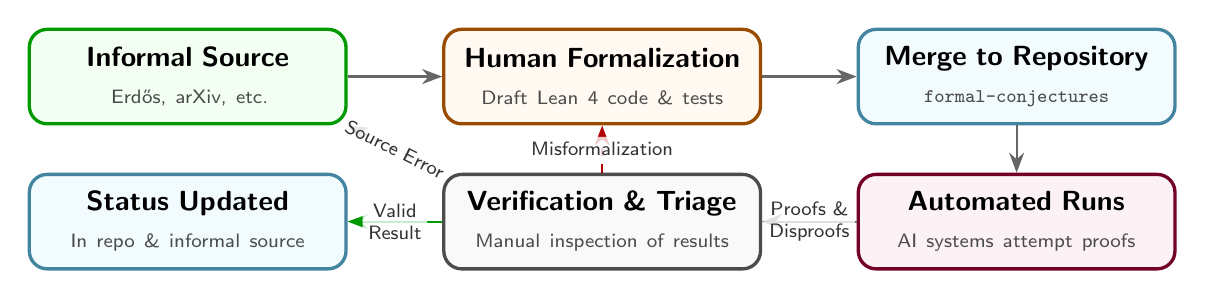
\begin{tikzpicture}[
    % Reduced vertical distance (0.6cm) and horizontal (1.2cm)
    node distance=0.6cm and 1.2cm,
    font=\sffamily,
    % Reduced minimum height to 1.2cm and inner sep to 6pt for vertical compactness
    flowbox/.style={rectangle, fill=#1!5, draw=#1!60!black, very thick, rounded corners=1.5ex, text width=3.6cm, minimum height=1.2cm, inner sep=6pt, align=center},
    % Arrow styles
    arrow/.style={thick, color=black!60, -{Stealth[scale=1.1]}},
    feedback/.style={thick, color=red!70!black, dashed, -{Stealth[scale=1.1]}},
    success/.style={thick, color=green!60!black, -{Stealth[scale=1.1]}},
    % Label styles (tightened inner sep)
    pathlabel/.style={font=\sffamily\scriptsize, text=black!80, align=center, fill=white, fill opacity=0.8, text opacity=1, inner sep=2pt, rounded corners=0.4ex}
]

    % ==========================================
    % ROW 1: The Forward Pipeline
    % ==========================================
    \node (source) [flowbox=green] {
        \textbf{Informal Source}\\[0.3ex]
        \color{black!70}\scriptsize Erdős, arXiv, etc.
    };

    \node (formalize) [flowbox=orange, right=of source] {
        \textbf{Human Formalization}\\[0.3ex]
        \color{black!70}\scriptsize Draft Lean~4 code \& tests
    };

    \node (repo) [flowbox=cyan, right=of formalize] {
        \textbf{Merge to Repository}\\[0.3ex]
        \color{black!70}\scriptsize \texttt{formal-conjectures}
    };


    % ==========================================
    % ROW 2: The Evaluation & Feedback Loop
    % ==========================================
    \node (eval) [flowbox=purple, below=of repo] {
        \textbf{Automated Runs}\\[0.3ex]
        \color{black!70}\scriptsize AI systems attempt proofs
    };

    \node (inspect) [flowbox=gray, below=of formalize] {
        \textbf{Verification \& Triage}\\[0.3ex]
        \color{black!70}\scriptsize Manual inspection of results
    };

    \node (status) [flowbox=cyan, below=of source] {
        \textbf{Status Updated}\\[0.3ex]
        \color{black!70}\scriptsize In repo \& informal source
    };


    % ==========================================
    % ROUTING ARROWS
    % ==========================================
    % 1. Forward Path
    \draw [arrow] (source.east) -- (formalize.west);
    \draw [arrow] (formalize.east) -- (repo.west);
    \draw [arrow] (repo.south) -- (eval.north);

    % 2. Into Triage
    \draw [arrow] (eval.west) -- (inspect.east) node[midway, pathlabel] {Proofs \&\\Disproofs};

    % 3. Feedback Loops (Red Dashed)
    \draw [feedback] (inspect.north) -- (formalize.south) node[midway, pathlabel] {Misformalization};

    % External Community Feedback (Diagonal)
    \draw [thick, dashed, color=black!50, -{Stealth[scale=1.1]}] (inspect.north west) -- (source.south east) node[midway, pathlabel, sloped] {Source Error};

    % 4. Success Path (Green)
    \draw [success] (inspect.west) -- (status.east) node[midway, pathlabel] {Valid \\ Result};

\end{tikzpicture}%
    }%
    \caption{Iterative pipeline for Formal Conjectures. Formalized statements are tested by periodic AI runs, solving problems or triggering a revision loop.}
    \label{fig:formalization_process}
\end{figure}

In Formal Conjectures, every contribution undergoes mandatory code review by humans with both Lean expertise and relevant mathematical domain knowledge.
While early contributions to the repository were written entirely by hand, the authoring process has evolved: most recent submissions use AI tooling, including agentic coding assistants and auto-formalization systems.
To facilitate high-quality AI-assisted contributions, the repository provides an \texttt{AGENTS.md} file with structured guidance for these tools.
Similarly, the review process increasingly leverages AI: reviewers use language models to cross-check formalizations against informal sources, and AlphaProof runs on submissions to catch potential misformalizations before merging.

Beyond this review process, we employ a number of additional strategies to mitigate the risk of misformalizations across the dataset.
Firstly, we employ and encourage a test-based design for definitions.
Any new definitions introduced should be accompanied by a suite of proven \texttt{test} lemmas and \texttt{API} statements that are designed to establish
expected behavior of the definition and mitigate the risk of edge-case errors.
Lean and \lstinline{Mathlib}'s tooling (for example \lstinline{decide}) can be employed to prove many of these \texttt{test} statements.
As of the \href{https://github.com/google-deepmind/formal-conjectures/releases/tag/bench-v1-lean4.27.0}{\texttt{bench-v1-lean4.27.0} release}, the repository contains \fcCountTest{} \texttt{test} statements and \fcCountAPI{} \texttt{API} statements, amounting to \fcCountInfraPct\% of the repository statements.

Secondly, automated theorem provers like AlphaProof regularly attempt proofs and disproofs across the repository (Figure \ref{fig:formalization_process}); manually inspecting these results primarily reveals misformalizations.
In contrast to test-based design, which proactively reduces the risk of edge-case errors, this retroactive approach is capable of unearthing misformalizations across all categories as described in Section~\ref{sec:misform}.
In addition, we use Gemini, AlphaProof, and other tools to automatically cross-check formalizations against their informal source texts, flagging potential discrepancies for human review.
Future work involves further automating these processes in GitHub CI in order to reduce the overhead of manual post-hoc fixes from the maintainers.

Thirdly, custom Lean linters built on Mathlib's framework enforce metadata and documentation standards across contributions.
These cover AMS classification tags, \lstinline{answer(sorry)} usage, problem category annotations, and module docstrings.

Finally, as Formal Conjectures has grown in stature, community engagement and proof/disproof attempts from external automated theorem provers have been increasingly valuable.
Furthermore, insights and corrections discovered through this process are actively upstreamed to the original sources, e.g., prompting the maintainer of the Erdős problems website to regularly clarify and adjust the informal problem statements.


\section{Benchmark Evaluation}\label{sec:experimental_evaluation}

\subsection{Evaluation Framework}\label{sec:experimental_setup}


\paragraph{Evaluation Paradigms.}
Formal Conjectures provides a dynamic, rigorous benchmark for advanced automated reasoning premised on novel mathematical insight as the ultimate intellectual hurdle for complex problems. We define two distinct setups:
\begin{enumerate}
    \item \textbf{Primary Goal: New Formal Proof Discovery.}
    Measuring AI's ability to discover formal proofs for open problems, these unsolved conjectures form a zero-contamination testbed for genuine mathematical discovery. Since no solutions exist in any training corpus, success provides a definitive signal of reasoning capabilities, removing the need for secretive evaluation sets common in other benchmarks.
    \item \textbf{Secondary Goal: Proof Auto-formalization.}
    This track provides a climbable benchmark treating the non-trivial translation of established mathematics into formal code as a distinct, rigorous challenge. It measures a model's ability to work with Lean~4 and Mathlib to formalize known arguments.
\end{enumerate}


\paragraph{Evaluating Open Problems.}
Evaluating open problems is definitive: as no formal solutions exist at release time, the first kernel-accepted proof provides a zero-contamination success signal.
However, since a proof may settle a misformalized statement rather than the intended problem, any result for an open conjecture triggers manual inspection for fidelity.


\paragraph{Fixed Benchmark Subsets.}
To enable stable model comparisons, we provide two frozen subsets of 100 problems each:
\texttt{FC100OpenSet1} (100 \texttt{research open} statements) and \texttt{FC100SolvedSet1} (100 \texttt{research solved} statements).
These subsets are defined in the repository files \texttt{FC100OpenSet1.lean} and \texttt{FC100SolvedSet1.lean}, which import exactly the corresponding theorem statements.
Because these files are compiled as part of the repository across all supported Lean versions, the problem sets remain fixed and comparable even as the repository evolves.
Further details on the construction of these subsets are in Appendix~\ref{sec:app_bench_lists}.


\paragraph{Correctness.}
Following established formal math benchmark methodologies \citep{minif2f21, putnambench24}, our evaluation leverages the Lean~4 kernel for an objective, rigorous, and automatable success criterion.
A proposed solution is a Lean proof term replacing the \lstinline{sorry} placeholder.
Solutions are correct if and only if accepted by the kernel without relying on forbidden axioms, such as \lstinline{sorry}.
This binary criterion eliminates human grading ambiguity and provides an indisputable ground truth.
While theoretically susceptible to foundational bugs in the Lean kernel or unintended axioms (e.g., a Lean Zulip thread\footnote{\url{https://leanprover.zulipchat.com/\#narrow/channel/270676-lean4/topic/Soundness.20bug.3A.20hasLooseBVars.20is.20not.20conservative/with/520153084}}, which mentions a now-fixed exploit), in practice, kernel-level verification provides the highest mathematical rigor.
Consequently, all evaluations are automatically verifiable, allowing results and proof terms to be shared publicly for transparent, reproducible research.


\paragraph{Versioning and Reproducibility.}\label{sec:versioning}
Evaluating on a living repository is challenging: dependency updates can alter statement semantics, and new Mathlib theorems may simplify problems.
To enable reproducible comparisons, we tag frozen benchmark snapshots using a two-part naming scheme: \texttt{bench-v$N$-lean4.$X$.$Y$}.
The \emph{bench version} \texttt{v$N$} identifies a fixed problem set; the \emph{Lean version} suffix pins the Mathlib tag (and hence Lean toolchain) against which statements compile and are evaluated.
Releases are issued every few months; when Lean versions bump, companion tags allow evaluating the same problem set against intermediate toolchains, e.g.\ \texttt{bench-v3-lean4.27.0}.
To preserve baselines, snapshots are immutable; misformalization fixes are never patched into existing versions but incorporated into the next (e.g., \texttt{bench-v$($N$+1)$}).


\paragraph{A Living Benchmark and Unified API.}
Outside the frozen subsets, the repository operates as a dynamic benchmark that exhibits useful evaluation dynamics over time.
As new conjectures are added, solved, or corrected by the community, it naturally self-adjusts its difficulty, expands, and improves.
The hardest problems remain open, pushing the frontier of automated reasoning.
Crucially, the repository acts as a unified API: researchers can submit formalized conjectures to a single centralized hub for simultaneous exposure to all evaluating AI systems.
This obviates the need to manually engage with individual provers, ensuring broad and concurrent attempts at mathematical discovery.

\begin{table}[t!]
  \caption{Proof coverage across all statement categories. \emph{Proved in repo}: the statement has a \lstinline{sorry}-free proof in the repository; \emph{Linked proof}: a proof is recorded via the \lstinline{@[formal\_proof]} attribute but is not present in the repository itself; \emph{With proof}: either of the above.}
  \label{tab:formal_proof_baseline}
  \centering
  \begin{tabular}{lrrrr}
    \toprule
    Category & Total & \multicolumn{3}{c}{Proof Status} \\
    \cmidrule(lr){3-5}
    & & Proved in repo & Linked proof & With proof \\
    \midrule
    \texttt{research\_solved} & 836 & 44 (5.3\%) & 101 (12.1\%) & 145 (17.3\%) \\
    \texttt{textbook} & 128 & 45 (35.2\%) & 3 (2.3\%) & 48 (37.5\%) \\
    \texttt{test} & 467 & 390 (83.5\%) & 3 (0.6\%) & 393 (84.2\%) \\
    \texttt{API} & 155 & 140 (90.3\%) & 0 & 140 (90.3\%) \\
    \midrule
    \textbf{Total} & 1586 & 619 (39.0\%) & 107 (6.7\%) & 726 (45.8\%) \\
    \bottomrule
  \end{tabular}
\end{table}



\paragraph{Open Problems Baseline.}
For the primary proof-discovery task on open problems, the baseline for the first tagged release \texttt{bench-v1-lean4.27} is $0\%$ for all systems: by definition, no formal proof exists for any \texttt{research open} statement at the time of tagging (problems with known solutions are reclassified as \texttt{research solved}).
Over time, these open statements may receive formal or informal proofs.
Proofs that expose a misformalization (Section~\ref{sec:misform}) rather than settling the intended problem trigger revisions incorporated into the next version.
In subsequent releases, interim-solved problems are reclassified to \texttt{research solved}, with formal solutions receiving the \lstinline{@[formal_proof]} attribute.
The new \texttt{research open} set combines remaining unsolved problems with new additions; thus, successive versions start with a baseline of $\geq 0\%$ solved statements and become increasingly more difficult.

\paragraph{Proof Auto-Formalization Baseline.}
For auto-formalization, the baseline is system-agnostic: we track all formal proofs contributed to the repository, regardless of origin.
These are tracked using the \lstinline{@[formal_proof]} attribute (Section~\ref{sec:formalization-methodology}), which records the proof system (\texttt{formal\_conjectures} for proofs within the repository, \texttt{lean4} for proofs in external Lean~4 projects such as Mathlib, or \texttt{other\_system} for proofs in Isabelle, Rocq, etc.) and links to the source.
Table~\ref{tab:formal_proof_baseline} summarizes the current state. Notably, 17.3\% of \texttt{research\_solved} statements have a known formal proof (5.3\% internal, 12.1\% linked externally).


\subsection{Illustrative Evaluation}\label{sec:experimental_results}


We provide illustrative evaluations, with setup and cost details in Appendix~\ref{sec:illustrative_evaluation}.


\begin{wraptable}{r}{0.45\textwidth}
  \vspace{-15pt}
  \caption{Results on the frozen \texttt{FC100SolvedSet1}.}
  \vspace{5pt}
  \label{tab:results_bench_table}
  \centering
  \small
  \begin{tabular}{lr}
    \toprule
    Method & Proved (\%) \\
    \midrule
    AlphaProof (1k sims)  & 45.0\% \\
    AlphaProof (16k sims) & 50.0\% \\
    DM prover agent (dev)       & 66.0\% \\
    \bottomrule
  \end{tabular}
  \vspace{-10pt}
\end{wraptable}


\paragraph{Frozen Evaluation Subsets.}
To ensure stable comparisons despite repository fluidity, we provide two frozen evaluation subsets, each containing 100 problems randomly sampled from the \texttt{bench-v1-lean4.27.0} tag: \texttt{FC100SolvedSet1} (proof auto-formalization) and \texttt{FC100OpenSet1} (proof discovery; 0\% baseline).
By definition, \texttt{FC100OpenSet1} currently remains at a definitive 0\% baseline across these evaluated methods, which highlights its status as a rigorous frontier for new discovery.
Results on \texttt{FC100SolvedSet1} (Table \ref{tab:results_bench_table}) demonstrate a clear, climbable signal across both compute and model capabilities.
To provide a diverse evaluation, we evaluate both a slightly improved version of the AlphaProof system used in the 2024 IMO \citep{AlphaProof25} and a development version of a DeepMind prover agent \citep{DMProverAgent26}.
These are different systems rather than incremental versions of the same architecture.
Utilizing a constrained tree-search-only inference setup on v6e TPUs, AlphaProof achieves a solve rate of 45\% on \texttt{FC100SolvedSet1} with a low compute configuration of 1,000 simulations per problem.
By increasing the compute budget to 16,000 simulations, the solve rate improves to 50\%, demonstrating a clear scaling signal.
We emphasize that these evaluations are conducted using tree-search inference only and do not utilize AlphaProof's test-time reinforcement learning (TTRL) mechanism, which generates a curriculum to learn from during the proof finding process through weight updates.
Furthermore, utilizing a newer, development version of the DeepMind prover agent, the solve rate increases to 66\%, illustrating that the benchmark effectively measures advancements across improved model architectures and methodologies.
Because running automated reasoning methods within Lean involves significant infrastructure overhead, we provide these specific systems as illustrative baselines to validate the benchmark's signal.
We encourage the community to report results against these subsets as well as the evolving main repository.


\section{Discussion}\label{sec:discussion}


\paragraph{Broader Benefits.}
Beyond its primary role, Formal Conjectures provides \textbf{precise mathematics} by enforcing a level of formal precision that clarifies the exact meaning of statements.
This creates a library of conjectures referenced unambiguously via unique file names and commit hashes, ensuring fixed and verifiable mathematical intent; unlike standard citations where generality or precision is often left to interpretation.
Furthermore, the benchmark serves as a compass for \textbf{Mathlib development}, as formalizing advanced conjectures reveals gaps in the existing library.
We address these via \texttt{FormalConjecturesForMathlib}, a directory of results continuously upstreamed to Mathlib. By identifying hard-to-state concepts, the repository both benchmarks reasoning and expands formalized mathematics.


\paragraph{Limitations.}
Problem selection faces a \textbf{scope bias} constrained by Mathlib's current coverage, which we mitigate somewhat via our \texttt{ForMathlib} directory. While some concepts remain hard to formalize, this limitation will diminish as Mathlib expands.
There is also a \textbf{selection bias} toward famous conjectures and Erd\H{o}s problems, resulting in a concentration of number theory and combinatorics; we plan to mitigate this by sourcing diverse arXiv preprints in areas like computer science and physics.
Focusing on open problems introduces a \textbf{misformalization risk} from subtle statement or source errors.
While mitigated via new methods in Section~\ref{sec:avoiding_misform}, these risks remain until a full proof is provided; fixing newly discovered errors may require revisions impacting historical comparisons.
The benchmark also faces \textbf{contamination challenges}: for solved problems, models may retrieve known arguments rather than reasoning from scratch; for open problems, zero-contamination is not permanent as future solutions enter training data.
Our living repository tracks these developments and reclassifies problems accordingly.
Finally, \textbf{verification and reproducibility} rely on the Lean~4 kernel's integrity; while the theoretical exploitability of foundational bugs or unintended axioms is a general challenge for formal systems, it remains the highest standard for rigor.
To ensure stable results despite the repository's evolution, we provide frozen, versioned subsets for standardized evaluation.


\paragraph{Future Work.}
As an active open-source project, we are committed to maintaining and extending Formal Conjectures with new problems, improved problems, and platform features; this ongoing commitment is reflected in the repository's steady growth since its initial release (see Figure~\ref{fig:repo_growth}).
See Appendix~\ref{sec:extended_discussion} for details on planned extensions, metadata improvements, and community features.



\section{Conclusion}\label{sec:conclusion}
We present \textbf{Formal Conjectures}, an evolving collection of mathematical problem statements formalized in Lean~4, including open conjectures.
Sourced from a diverse range of mathematical literature and areas, the benchmark provides broad coverage as an evaluation framework for AI systems' capabilities in formal math.
By providing a zero-contamination testbed of research-level problems alongside a substantial set for proof auto-formalization, we establish a rigorous environment for evaluating AI for formal mathematical research.
Crucially, to ensure stable and reproducible model comparisons as the repository evolves, we complement this dynamic dataset with versioned, frozen evaluation subsets.
We hope the work can drive the expansion of formalized math: both through its living repository and the continuous upstreaming of new definitions to Mathlib, as well as serve as a high-fidelity benchmark that bridges the gap between human mathematical expertise and automated formal reasoning.
Ultimately, we believe this resource will not only measure current progress but also help accelerate the frontier of formal mathematical discovery.



\begin{ack}
We thank all contributors who have contributed to the repository since it was released as open source, among them
Abel Do\~{n}ate,
Aditya Ramabadran,
Amogh Parab,
Anirudh Rao,
Anthony Wang,
Ayush Debnath,
Bhavik Mehta,
Bolton Bailey,
Cong Lu,
Daniel Chin,
Felix Pernegger,
Franz Huschenbeth,
James Jordan,
Jean-Guillaume Durand,
Jofre Costa,
Junseok Lee,
Junyan Xu,
Madhu Shree Aravindan,
Mario Krenn,
Martin Bruse,
Michael Rothgang,
Mirek Ol\v{s}\'{a}k,
Ralf Stephan,
Reklle,
Seewoo Lee,
The bbchallenge Collaboration (bbchallenge.org),
Wojciech Nawrocki,
Yan Yablonovskiy,
Yoh Tanimoto,
Yongxi Lin,
Zeyu Zheng,
and Zhen Ning David Liu.
A full list of contributors is available at \url{https://github.com/google-deepmind/formal-conjectures/graphs/contributors}.
Additionally, we thank Swarat Chaudhuri, George Tsoukalas, Anton Kovsharov, Henryk Michalewski, Edward Lockhart, and Goran Žužić for helpful discussions and support running experiments.
\end{ack}

\bibliographystyle{plainnat}
\bibliography{all}


\appendix

\newpage

\section*{Supplementary Material}

Here, we include various supplementary details.

\section{Formal Conjectures Details}\label{sec:app_formal_conjectures}


\subsection{Source and AMS Classification Tables}\label{sec:app_source_ams_tables}

Note that a single source problem typically gives rise to multiple formal statements due to variants (e.g., special cases, generalizations, solved sub-problems, and test lemmas). We explicitly allow and encourage the inclusion of multiple alternative formalizations for a single informal claim to capture different mathematical perspectives or resolutions of ambiguity; thus, the counts in this table reflect formal statements, not distinct source problems.

\begin{table}[h]
    \caption{Number of formal statements by source collection, split by category. A single source problem may yield multiple statements (variants, special cases, tests).}
    \label{tab:problems-by-collection}
    \centering
    \begin{tabular}{lrrrr}
    \toprule
    \textbf{Source Collection} & \textbf{Total} & \textbf{Research Open} & \textbf{Research Solved} & \textbf{All Other} \\
    \midrule
    Erd\H{o}s Problems & 1318 & 551 & 551 & 216 \\
    Wikipedia & 476 & 208 & 113 & 155 \\
    Green's Open Problems & 175 & 83 & 73 & 19 \\
    Papers & 131 & 65 & 25 & 41 \\
    Open Quantum Problems & 125 & 35 & 13 & 77 \\
    Written on the Wall II & 110 & 13 & 12 & 85 \\
    OEIS & 105 & 22 & 6 & 77 \\
    arXiv & 56 & 13 & 13 & 30 \\
    MathOverflow & 53 & 12 & 9 & 32 \\
    All other sources & 66 & 27 & 21 & 18 \\
    \midrule
    \textbf{Total} & \textbf{2615} & \textbf{1029} & \textbf{836} & \textbf{750} \\
    \bottomrule
    \end{tabular}
\end{table}


Table~\ref{tab:ams-breakdown} shows the distribution of statements across AMS subject classifications.
Other notable areas beyond number theory and combinatorics include quantum theory, linear algebra, and algebraic geometry.

\begin{table}[h]
    \caption{Top 10 AMS subject classifications by number of statements in Formal Conjectures.}
    \label{tab:ams-breakdown}
    \centering
    \begin{tabular}{lr}
    \toprule
    \textbf{AMS Subject Classification} & \textbf{Statements} \\
    \midrule
    Number theory & 1545 \\
    Combinatorics & 923 \\
    Quantum theory & 174 \\
    Linear and multilinear algebra; matrix theory & 140 \\
    Information and communication, circuits & 96 \\
    Convex and discrete geometry & 93 \\
    Algebraic geometry & 80 \\
    Geometry & 56 \\
    Field theory and polynomials & 53 \\
    Group theory and generalizations & 42 \\
    \bottomrule
    \end{tabular}
\end{table}


\subsection{The \texorpdfstring{\lean{answer(sorry)}}{answer(sorry)} Mechanism in Detail}\label{sec:app_answer_sorry}

Problems requiring a solution are formalized using \lean{answer( )}, a custom Lean term elaborator.
Concretely, a problem like \enquote{What is the smallest $n$ such that $P(n)$?} is formalized as:
\begin{leancode}
theorem smallest_n : IsLeast {n : ℕ | P n} answer(sorry) := by
  sorry
\end{leancode}
As usual, \lean{sorry} is a placeholder which must be filled in order to claim that a problem is solved, but now there are two of them.
If the solution is known, then \lean{answer(sorry)} is replaced in the statement with \lean{answer(42)}.
This mechanism allows our statements to include computational conjectures where discovering the answer is the primary challenge and verification is routine.

Crucially, while providing a proof simply requires finding any way to replace \lean{:= sorry} with a valid term, providing an answer is a fundamentally different task: it requires evaluating mathematical meaning to determine the correct value.
Lean's type checker can verify that a proposed answer leads to a valid proof, but it cannot judge whether the answer itself is mathematically meaningful---that remains a job for human mathematicians or AI systems with genuine mathematical reasoning capabilities.

There are a number of advantages to using the \lean{answer( )} wrapper over directly writing a solution or a bare \lean{sorry} placeholder:
\begin{itemize}
\item It makes clear which part of the formalization corresponds to the solution; this allows the solution to be masked from \lean{research solved} statements in order to evaluate agents. This can either be done by inspecting the metadata inserted in the Lean term, or more pragmatically, by a simple regex replacement.
\item
    It provides some protection against Lean's flexible elaboration; a problem stated as \lean{1 / 2 * 2 = sorry} could be solved by replacing the \lean{sorry} with either \lean{(0 : ℕ)} or \lean{(1 : ℚ)},
    as by default, Lean only infers the type of an equality after analyzing both sides.
    This is clearly undesirable; we do not want the meaning of our questions to change depending on the answer provided!
    Stating the problem instead as \lean{1 / 2 * 2 = answer(sorry)} protects against this, as the \lean{answer} elaborator postpones analysis which forces Lean to decide the type of the equality before seeing the solution.
\item It forces the statement to be written in such a way that does not pre-assume what the solution is.
\end{itemize}

\subsubsection{Propositional Solutions}

A particularly common use case arises when the truth value of a proposition $P$ is itself unknown, i.e. when the problem can be phrased as a question: "Is it true that...".
In this case, \lean{answer(sorry)} serves as a propositional placeholder that should be replaced with either \lean{True} or \lean{False}:
\begin{leancode}
theorem is_P_true : answer(sorry) ↔ P := by
  sorry
\end{leancode}
Replacing \lean{answer(sorry)} with \lean{True} amounts to conjecturing that $P$ holds (and the solver must prove $P$),
while replacing it with \lean{False} amounts to conjecturing that $P$ fails (and the solver must disprove $P$).
This pattern is widely used throughout the repository for open problems where even the expected truth value is uncertain.

For the convenience of evaluating solver systems that are capable of filling proofs only,
when \lean{answer(sorry)} is detected to be used propositionally in this way, it elaborates to \lean{True} under its default settings.
This permits these systems to decide the proposition by either proving or disproving the statement, rather than by filling the placeholder.


\subsection{The \enquote{for Mathlib} Pattern}\label{sec:app_for_mathlib}

It is typical when undertaking formalization projects to discover missing (and often trivial) results that seem suitable for Mathlib.
Contributing these results to Mathlib is of course the natural resolution, but this has a number of downsides:
\begin{itemize}
\item  New conjectures that depend on these results find themselves at the end of a long dependency chain; the missing results must undergo Mathlib review, the merged change must land in a monthly Mathlib release, and the Formal Conjectures repository must be upgraded to that release
\item Some results may be too specialized for Mathlib, and a Mathlib contribution would require generalizing these immediately.
\item When the results entail a whole new mathematical development, it may take time for the Mathlib community to find the right abstractions and evolve said development into the right shape. Bypassing the dependency chain mentioned above allows much of this evolution to happen more rapidly outside of Mathlib.
\end{itemize}

The Lean community has widely adopted the pattern of creating a \texttt{ForMathlib} directory as a staging ground for such results, the oldest example of which being \href{https://github.com/leanprover-community/lean-liquid/tree/master/src/for\_Mathlib}{the \texttt{for\_mathlib} directory} in the \enquote{liquid tensor experiment}\footnote{\url{https://github.com/leanprover-community/lean-liquid}}.
The formal-conjectures project's \texttt{FormalConjecturesForMathlib} directory follows this pattern, and contains 88 files with results such as natural and logarithmic density of sets of natural numbers (with proofs of basic properties like monotonicity and the density of even numbers), arithmetic progressions and AP-free sets, hypergraph Ramsey numbers, Turing machines and busy beaver halting numbers, perfect powers with a decidability instance, VC dimension in abelian groups, Latin squares and transversals, and a library of graph invariants including the Wiener and Szeged indices, the Lov\'{a}sz theta function, and the Havel--Hakimi residue.
Over time, these results are asynchronously contributed upstream to Mathlib.

\subsection{Misformalization Taxonomy}\label{sec:app_misform_taxonomy}

Misformalizations can be categorized roughly as follows, with the level shown in parentheses.\footnote{Pull request (PR) numbers refer to the repository at \url{https://github.com/google-deepmind/formal-conjectures}; Erd\H{o}s Problem discussions are at \url{https://www.erdosproblems.com}.}
\begin{itemize}
    \item \textbf{Syntactic (1)}: where the formalizer misses a subtlety in the way Lean parses a piece of syntax. For example, this could be missing brackets changing the meaning of an expression in unexpected ways; see PR~\#1338.
    \item \textbf{Semantic (1)}: where the formalizer misses a subtlety in the way that Lean represents types or operators. For example, the natural numbers in Lean contain $0$ and have truncated subtraction; see PRs~\#349, \#1259, \#1262.
    \item \textbf{Misrepresentation (1)}: where the formalizer formally misrepresents aspects of the informal statement during translation. For example, the use of incorrect quantifiers, the use of incorrect logical connectives, or the failure to include hypotheses which are present in the source text; see PRs~\#1164, \#1156.
    \item \textbf{Implicit conventions (2)}: where the source text assumes domain expertise and does not explicitly include certain hypotheses or conventions. For example, in analytic number theory, questions about the magnitude of a set of numbers are often implicitly asymptotic; see PRs~\#2136, \#1151.
    \item \textbf{Reporting (3)}: where the statement changes in the literature through repetition, usually as the result of typos; see Erd\H{o}s Problem~918 discussion.
    \item \textbf{Mathematical (3)}: where the source text is clearly not as intended or contains genuine mathematical errors; see Erd\H{o}s Problem~728 discussion.
\end{itemize}

\begin{table}[H]
    \centering
    \caption{Number and proportion of misformalizations across categories.}
    \label{tab:misform_table}
    \begin{tabular}{llc}
        \textbf{Level} & \textbf{Category} & \textbf{Number of misformalizations} \\
        \toprule
        \multirow{3}{*}{Translation} & Syntactic & 9 (3.09\%)\\
        \cmidrule{2-3}
        & Semantic & 103 (35.40\%)\\
        \cmidrule{2-3}
        & Misrepresentation & 140 (48.11\%) \\
        \midrule
        Underspecified & Implicit conventions & 23 (7.90\%) \\
        \midrule
        \multirow{2}{*}{Source} & Reporting & 15 (5.15\%)\\
        \cmidrule{2-3}
        & Mathematical & 1 (0.34\%) \\
        \bottomrule
    \end{tabular}
\end{table}

\subsection{Misformalization Examples}\label{sec:app_misformalization_examples}

This section contains the misformalization examples, mentioned in Section~\ref{sec:misform}. 

\subsubsection{Syntactical Errors}

An example of a syntactical error involving the correction of misplaced parentheses is shown in Figure \ref{fig:misform_syntactic_erdos1054}.

\begin{figure}[h]
    \centering
    \begin{minted}{diff}
  /-- Let $f(n)$ be the minimal integer $m$ such that $n$ is the sum of the 
  $k$ smallest divisors of $m$ for some $k\geq 1$. Is it true that 
  $\limsup f(n)/n=\infty$? -/
  @[category research open, AMS 11]
  theorem erdos_1054.parts.iii : (∃ (A : Set ℕ), A.HasDensity 1 ∧
-      atTop.limsup (fun n ↦ (f n : EReal) / n) = ⊤) ↔ answer(sorry) := by
+      atTop.limsup (fun n ↦ (f n : EReal) / n = ⊤)) ↔ answer(sorry) := by
  sorry
    \end{minted}
    \caption{Code diff showing an example of a syntactical error, and the correction of parentheses.}
    \label{fig:misform_syntactic_erdos1054}
\end{figure}

\subsubsection{Semantic Errors}

Figures 
\ref{fig:misform_semantic_coeffs}, \ref{fig:misform_semantic_growth} and \ref{fig:misform_semantic_covering} illustrate various semantic errors encountered during formalization.

\begin{figure}[h]
    \centering
    \begin{minted}{diff}
  /-- `Polynomial.HasOddCoeffs f` means that all coefficients of 
  `f : Polynomial ℤ` are odd. -/
  def Polynomial.HasOddCoeffs (f : Polynomial ℤ) : Prop :=
-   ∀ i : ℕ, Odd (f.coeff i)
+   ∀ i ∈ f.support, Odd (f.coeff i)
    \end{minted}
    \caption{Code diff showing an example of a semantic error, with the fix requiring quantification over the support of the polynomial.}
    \label{fig:misform_semantic_coeffs}
\end{figure}

\begin{figure}[h]
    \centering
    \begin{minted}{diff}
  /-- A group `HasPolynomialGrowth` if there exists a finite generating set 
    such that the growth function is bounded above by a polynomial. -/
  def HasPolynomialGrowth (G : Type*) [Group G] : Prop :=
    ∃ (S : Set G), Set.Finite S ∧ Subgroup.closure S = ⊤ ∧
      ∃ (C : ℝ) (d : ℕ), C > 0 ∧
-     ∀ n : ℕ, (GrowthFunction S n : ℝ) ≤ C * (n : ℝ) ^ d
+     ∀ n > 0, (GrowthFunction S n : ℝ) ≤ C * (n : ℝ) ^ d
    \end{minted}
    \caption{Code diff showing an example of a semantic error, where the formalization had failed to account for behavior at the natural number $0$.}
    \label{fig:misform_semantic_growth}
\end{figure}

\begin{figure}
    \centering
    \begin{minted}{diff}
+ /-- An exact covering of a group `G` is a finite collection of subgroups 
+ `{H_1, ..., H_k}` and representative `{g_1, ..., g_k}` such that the 
+ cosets `g_iH_i` are pairwise disjoint and their union covers `G`.
+ 
+ Note that this differs from `Partition (α := Subgroup G)` because the 
+ covering condition there invokes `Subgroup.sup` which is subgroup generation 
+ and thus stronger than union. This definition is easier to use in this 
+ context than the alternative `Partition (α := Set G)`, which lacks
+ subgroup definitions such as `Subgroup.index`. -/
+ structure Group.ExactCovering (G : Type*) [Group G] (ι : Type*) [Fintype ι] where  
+   parts : ι → Subgroup G
+   reps : ι → G
+   nonempty (i : ι) : (parts i : Set G).Nonempty
+   disjoint : (Set.univ (α := ι)).PairwiseDisjoint 
+     fun (i : ι) ↦ reps i • (parts i : Set G)
+   covers : ⋃ i, reps i • (parts i : Set G) = Set.univ

  /--
  If `G` is a group then can there exist an exact covering of `G` by more than 
  one cosets of different sizes? (i.e. each element is contained in exactly 
  one of the cosets.)
  -/
  @[category research open, AMS 20]
  theorem erdos_274 (G : Type*) [Group G] (hG : 1 < ENat.card G) :
-     (∃ (P : Partition (⊤ : Subgroup G)),
-       1 < P.parts.ncard ∧
-       (∀ A ∈ P.parts, ∃ᵉ (s : G) (H : Subgroup G), s • (H : Set G) = A) ∧
-       P.parts.Pairwise fun A B ↦ #A ≠ #B) ↔ answer(sorry) := by
+     (∃ (ι : Type*) (_ : Fintype ι) (P : Group.ExactCovering G ι),
+       1 < Fintype.card ι ∧ (Set.range P.parts).Pairwise fun A B ↦ #A ≠ #B) ↔ 
+         answer(sorry) := by
  sorry
    \end{minted}
    \caption{Code diff showing an example of a semantic error, where the formalization missed the subtlety that \lean{Partition} invokes \lean{sup} for the covering condition, which means something different for subgroups than for sets.}
    \label{fig:misform_semantic_covering}
\end{figure}

\clearpage 

\subsubsection{Misrepresentation Errors} 

Figure \ref{fig:misform_misrep_giuga} provides an example of a misrepresentation error where a hypothesis from the informal text was omitted, and Figure \ref{fig:misform_misrep_quantifier} shows an error involving incorrect quantification.

\begin{figure}[h]
    \centering
    \begin{minted}{diff}
  /--
- A (weak) Giuga number is a number $n$ such that
+ A (weak) Giuga number is a composite number $n$ such that
  $$\sum_{i=1}^{n - 1}i^{\varphi(n)} \equiv -1\pmod{n}$$.
  -/
  def IsWeakGiuga (n : ℕ) : Prop :=
-     2 ≤ n ∧ ¬ n.Prime ∧ n ∣ 1 + ∑ i ∈ Finset.Ioo 0 n, i ^ φ n
+     n.Composite ∧ n ∣ 1 + ∑ i ∈ Finset.Ioo 0 n, i ^ φ n
    \end{minted}
    \caption{Code diff showing an example of a misrepresentation error, where the formalization was missing a hypothesis that was present in the informal text. }
    \label{fig:misform_misrep_giuga}
\end{figure}

\begin{figure}[h]
    \centering
    \begin{minted}{diff}
  @[category research open, AMS 11]
  theorem erdos_944 :
-     (∀ k ≥ 4, ∀ r ≥ 1, ∃ (G : SimpleGraph V), G.IsErdos944 k r) ↔ 
-       answer(sorry) := by
+     (∀ k ≥ 4, ∀ r ≥ 1, ∃ (V : Type u) (G : SimpleGraph V), G.IsErdos944 k r) ↔ 
+       answer(sorry) := by
  sorry
    \end{minted}
    \caption{Code diff showing an example of a misrepresentation error, where the vertex type \lean{V} was incorrectly quantified. In the old version \lean{V} was a section variable and thus appeared out of the scope of the existential quantifier.}
    \label{fig:misform_misrep_quantifier}
\end{figure}

\subsubsection{Implicit Conventions}

Examples of errors stemming from implicit conventions in the source material can be seen in Figures \ref{fig:misform_implicit_asymptotic} and \ref{fig:misform_implicit_induced}.

\begin{figure}[h]
    \centering
    \begin{minted}{diff}
  @[category research open, AMS 11]
  theorem erdos_510 :
      answer(sorry) ↔ ∃ (c : ℝ) (hc : 0 < c),
-       ∀ N > 0, ∀ (A : Finset ℕ), 0 ∉ A → #A = N →
+       ∀ᶠ N in atTop, ∀ (A : Finset ℕ), 0 ∉ A → #A = N →
        ∃ θ, ∑ n ∈ A, cos (n * θ) < -c * sqrt N := by
    sorry
    \end{minted}
    \caption{Code diff showing an example of an implicit convention, where the source\protect\footnotemark\ implicitly assumes that the inequality holds for sufficiently large $N$. This is a common implicit convention across analytic number theory where one is typically interested in the asymptotic behavior of functions or sequences of natural numbers.}
    \label{fig:misform_implicit_asymptotic}
\end{figure}
\footnotetext{\url{https://www.erdosproblems.com/510}}
\newpage
\begin{figure}[h]
    \centering
    \begin{minted}{diff}
  @[category research open, AMS 5]
  theorem erdos_128 :
-     ((∀ (G' : G.Subgraph) [Fintype G'.verts] [Fintype G'.edgeSet],
-         letI n := Fintype.card V;
-         2 * G'.verts.toFinset.card ≥ n →
-         50 * G'.edgeSet.toFinset.card > n^2) → ¬ (G.CliqueFree 3))
+     ((∀ (V' : Set V),
+       2 * V'.ncard ≥ Fintype.card V →
+         50 * (G.induce V').edgeSet.ncard > Fintype.card V ^ 2) → ¬(G.CliqueFree 3))
    ↔ answer(sorry) := by
  sorry
    \end{minted}
    \caption{Code diff showing an example of an implicit convention, where the source\protect\footnotemark\ wrote ``subgraph" rather than ``induced subgraph". The comments\protect\footnotemark\ demonstrate that the problem is trivial if one does not restrict to induced subgraphs, which is why we class this as implicit convention. It might also be considered to be a reporting error since the original paper explicitly writes ``induced subgraph", \cite[p. 344]{Erdos93}.}
    \label{fig:misform_implicit_induced}
\end{figure}
\addtocounter{footnote}{-1}\footnotetext{\url{https://www.erdosproblems.com/history/128}}
\addtocounter{footnote}{1}\footnotetext{\url{https://www.erdosproblems.com/forum/thread/128}}
 
\subsubsection{Reporting Errors}

Figure \ref{fig:misform_reporting_erdos918} demonstrates a reporting error caused by ambiguities in the historical source material regarding induced subgraphs.

\begin{figure}[H]
    \centering
    \begin{minted}{diff}
  /-- Is there a graph with $\aleph_2$ vertices and chromatic number $\aleph_2$ such that every
  subgraph on $\aleph_1$ vertices has chromatic number $\leq\aleph_0$? -/
  -- Formalisation note: source material [ErHa68b] uses only induced subgraphs
  @[category research open, AMS 5]
  theorem erdos_918.parts.i :
      (∃ (V : Type u) (G : SimpleGraph V), #V = ℵ_ 2 ∧ G.chromaticCardinal = ℵ_ 2 ∧
-       ∀ (W : Set V) (_ : #W = ℵ₁), (G.induce W).chromaticCardinal = ℵ₀) ↔
+       ∀ (W : Set V) (_ : #W = ℵ₁), (G.induce W).chromaticCardinal ≤ ℵ₀) ↔
      answer(sorry) := by
    sorry
    \end{minted}
    \caption{Code diff showing an example of a reporting error between an internal draft formalization of the problem. This problem appears in \cite{EH68} and \cite{Erdos69}. In the former citation the explicit use of $\leq \aleph_0$ is used, while this does not appear in the latter citation. This ambiguity was only clarified post draft formalization with the discovery of trivial solutions -- in the (non-induced) subgraph case by the website comments\protect\footnotemark\ and by AlphaProof in the induced subgraph case. Note also that \cite{EH68} explicitly writes \emph{induced} subgraph while \cite{Erdos69} and the website do not.}
    \label{fig:misform_reporting_erdos918}
\end{figure}
\footnotetext{\url{https://www.erdosproblems.com/forum/thread/918}}


\section{Experimental Evaluation Details}\label{sec:app_experimental_evaluation}


\subsection{Frozen Subsets}\label{sec:app_bench_lists}

The frozen subsets \texttt{FC100SolvedSet1} and \texttt{FC100OpenSet1} consist of 100 problems each, sampled uniformly at random from statements in the \texttt{research solved} and \texttt{research open} categories, respectively.
They are defined by the files \path{FormalConjectures/Subsets/FC100OpenSet1.lean} and \path{FormalConjectures/Subsets/FC100SolvedSet1.lean} in the repository, which import exactly the corresponding theorem statements.
These files are compiled as part of every tagged release, ensuring that the problem sets remain well-defined and their statements compile correctly across all supported Lean versions.

The subset names (e.g., \texttt{FC100OpenSet1}) are \emph{orthogonal} to the repository's release tags (\texttt{bench-v$N$-lean4.$X$.$Y$}, see Section~\ref{sec:versioning}).
When the bench version $N$ stays the same and only the Lean version changes (e.g., from \texttt{bench-v1-lean4.27.0} to \texttt{bench-v1-lean4.29.0}), the problem set is guaranteed to contain the same statements; the new tag only ensures compilation against the updated Lean toolchain and Mathlib.
When the bench version increments (e.g., from \texttt{bench-v1} to \texttt{bench-v2}), statements in an existing set may receive fixes (e.g., corrected misformalizations) or category updates (e.g., an \texttt{open} problem reclassified as \texttt{solved}), but the \emph{membership} of the set remains stable: no problems are added or removed.
For full reproducibility, results should specify both the set name and the release tag, e.g., \texttt{FC100SolvedSet1@bench-v1-lean4.27.0}.

In the future, we plan to release additional sets (e.g., \texttt{FC100SolvedSet2}, \texttt{FC500OpenSet1}) that may contain entirely different problems, enabling targeted evaluations at different scales or difficulty levels while preserving earlier sets.


\subsection{Illustrative Evaluation Details}\label{sec:illustrative_evaluation}


As noted in Section \ref{sec:experimental_results}, our evaluations focus on demonstrating the benchmark’s utility and its sensitivity to scaling.
For all systems, a solution is correct if and only if the Lean~4 kernel accepts the proof term without relying on forbidden axioms.


\paragraph{AlphaProof Setup.}
We evaluated a slightly updated version of AlphaProof \citep{AlphaProof25}, with tree-search inference, without the test-time reinforcement learning loop.
As reported in Table \ref{tab:results_bench_table}, we distinguish between two compute configurations for AlphaProof to demonstrate the benchmark's sensitivity to search budget: 1k sims utilizes 1,000 simulations and 2 attempts per problem (approximately 0.1 TPUh on v6e TPUs); and 16k sims and 2 attempts (approximately 1.6 TPUh on v6e TPUs).


\paragraph{DeepMind Prover Agent Setup.}
The DeepMind prover agent \citep{DMProverAgent26} results were obtained using a development version of the method under active experimentation.
Based on current API pricing, this evaluation costs up to \$100 per problem.



\section{Extended Discussion}\label{sec:extended_discussion}

\subsection{Future Work}\label{sec:app_future_work}

We plan to continuously extend Formal Conjectures with new problems unblocked by newly added Mathlib definitions or from community contributions.
While our implementation uses Lean~4, the methodology is language-agnostic and portable to systems like Isabelle or Rocq should they develop comparable library support. We will also track future Lean updates to maintain ecosystem compatibility.
To better evaluate the difficulty and impact of conjectures, we plan to extend the metadata by recording when a conjecture was first proposed.
This objective metric will enable users to filter for long-standing open problems versus contemporary questions.
However, since difficulty and importance are often subjective, we also propose an interactive interface where the community can share insights.
Users will be able to vote on a conjecture's perceived difficulty, its mathematical significance, and their conviction regarding its truth value
(e.g., True, False, or independent of ZFC).

Furthermore, references to the mathematical literature are currently handled inconsistently across the repository, often requiring duplication in each file. We plan to improve this by centralizing reference management in future iterations.

This vision is being integrated into an accompanying website\footnote{\url{https://google-deepmind.github.io/formal-conjectures/}} for the repository.
The website already serves as a frontend for the benchmark, allowing users to explore the source code, view \LaTeX-rendered docstrings, and search, sort, or filter conjectures.
It also contains metadata recording when a \lstinline[language={}]{research open} problem gets solved or when a \lstinline[language={}]{research solved} problem receives a formal proof; in the future, we plan to make these changes more prominently visible.

Moving forward, we plan to expand this platform into a collaborative hub with interactive community features, including a public leaderboard to track successful AI-based solutions and recognize groups taking on these problems.



\end{document}
